\documentclass{article}
\usepackage{graphicx}
\graphicspath{ {./images/} }
\usepackage{tikz}

\begin{document}
	
	\title{GUI based game: Racket}
	\author{Nikita Melentjevs, Julian Michelsen}
	
	\maketitle
	
	\section{requirements}
	Create a Gui based game using racket, accepting user needs and requirements, 
	visually pleasing functional, bug free final product. \newline
	refining of the problem and posing possible solutions.
	\begin{itemize}
		\item Create a character for the player to control?
		\item Create a level scape for the player to navigate?
		\item Create some way to level up and increase difficulty?
		\item Create enemies of some sort/obstacles?
		\item Create an initial menu screen for the player to choose options and such.
	\end{itemize}
	Possible Solutions:
	\begin{itemize}
		\item portal game
		\item shooter game
		\item geometry dash
	\end{itemize}
	\section{Design}
	Our game is an open-loop system as it relies on the input of the user to create 
	any sort of desired output:
	\begin{itemize}
		\item Our input system is the keyboard where keyboard commands are entered, as well as the cursor and cursor clicks on the initial menu screen.
		\item The controller is the update function, where time is taken into consideration and the user inputs are taken into consideration.
		\item The response is the movement of the player on the GUI.
	\end{itemize}
	\newpage
	\subsection{Top Down Approach}
	Our game is being created with top down design: \\
	where our approach is as follows: \\
	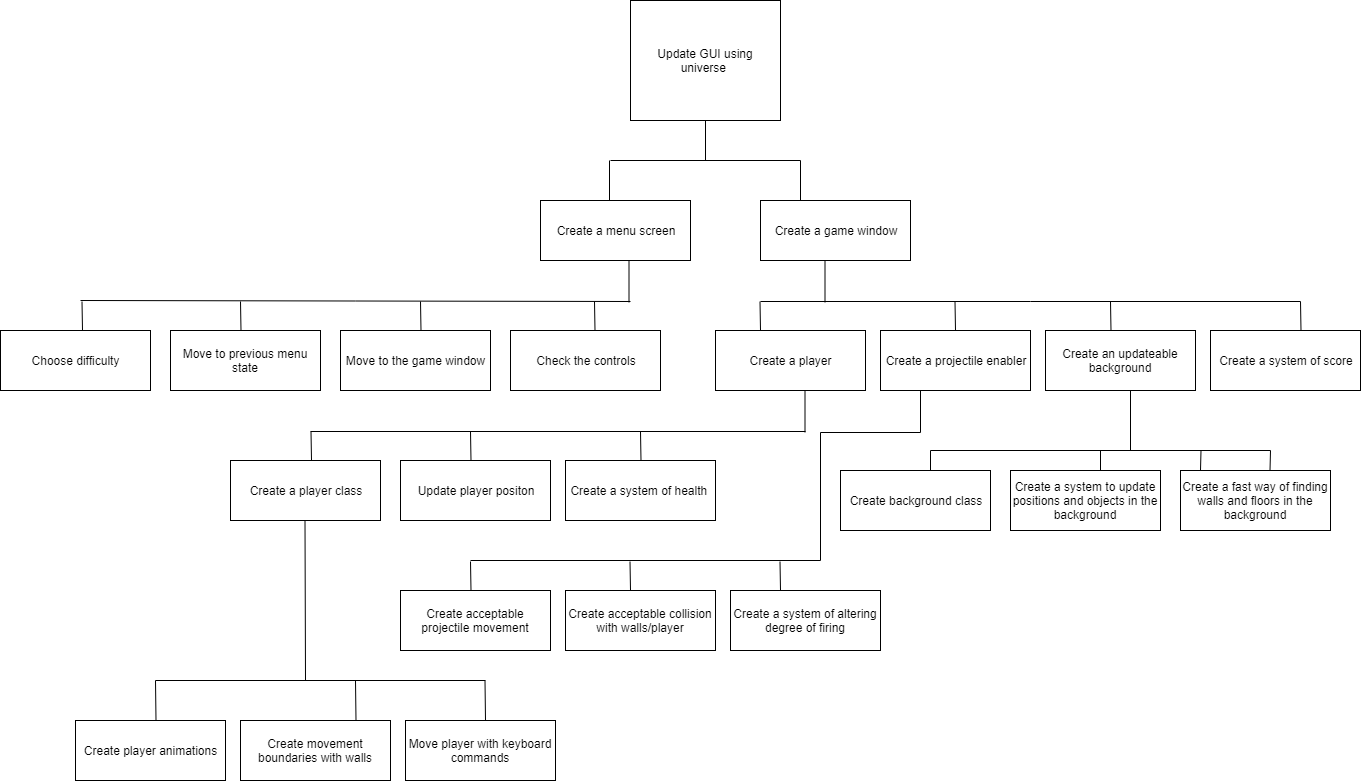
\includegraphics[scale=0.35]{blah1}
	\subsection{Use Cases}
	\begin{itemize}
		\item Create movement through keyboard clicks
		\item Fire a projectile through keyboard clicks
		\item Create a background that looks reasonable
		\item Create enemies to avoid
		\item Create a system of health
		\item Create a system of score
		\item Create animations for the player
		\item Create an acceptable leveling system
	\end{itemize}
	\subsection{UML Class Diagram}
	Write your subsection text here.
	\subsection{Different Data Structures}
	Lists, Hash tables, sets
	\subsection{FSM's}
	\textbf{Movement through Keyboard Click:} where F represents a check-falling function \\
	Blank line represents time passing.
	\medskip
	\begin{center}
		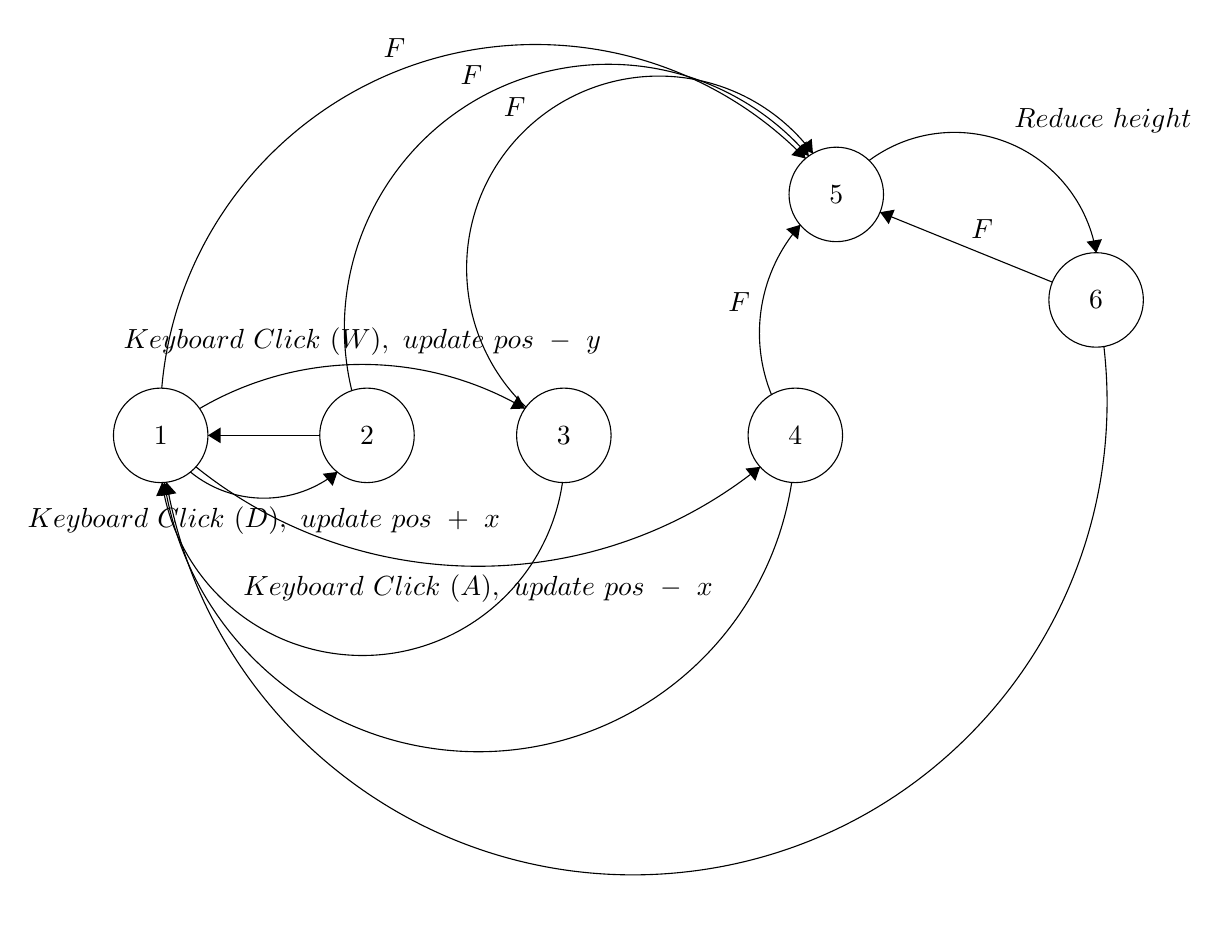
\begin{tikzpicture}[scale=0.2]
		\tikzstyle{every node}+=[inner sep=0pt]
		\draw [black] (8.9,-26.1) circle (3);
		\draw (8.9,-26.1) node {$1$};
		\draw [black] (22,-26.1) circle (3);
		\draw (22,-26.1) node {$2$};
		\draw [black] (34.5,-26.1) circle (3);
		\draw (34.5,-26.1) node {$3$};
		\draw [black] (49.2,-26.1) circle (3);
		\draw (49.2,-26.1) node {$4$};
		\draw [black] (51.8,-10.8) circle (3);
		\draw (51.8,-10.8) node {$5$};
		\draw [black] (68.3,-17.5) circle (3);
		\draw (68.3,-17.5) node {$6$};
		\draw [black] (20.126,-28.416) arc (-50.62992:-129.37008:7.372);
		\fill [black] (20.13,-28.42) -- (19.19,-28.54) -- (19.82,-29.31);
		\draw (15.45,-30.59) node [below] {$Keyboard\mbox{ }Click\mbox{ }(D),\mbox{ }update\mbox{ }pos\mbox{ }+\mbox{ }x$};
		\draw [black] (11.368,-24.399) arc (120.36918:59.63082:20.436);
		\fill [black] (32.03,-24.4) -- (31.59,-23.56) -- (31.09,-24.43);
		\draw (21.7,-21.09) node [above] {$Keyboard\mbox{ }Click\mbox{ }(W),\mbox{ }update\mbox{ }pos\mbox{ }-\mbox{ }y$};
		\draw [black] (46.966,-28.1) arc (-51.17683:-128.82317:28.577);
		\fill [black] (46.97,-28.1) -- (46.03,-28.21) -- (46.66,-28.99);
		\draw (29.05,-34.91) node [below] {$Keyboard\mbox{ }Click\mbox{ }(A),\mbox{ }update\mbox{ }pos\mbox{ }-\mbox{ }x$};
		\draw [black] (8.967,-23.103) arc (-184.8842:-315.85892:23.853);
		\fill [black] (49.85,-8.52) -- (49.65,-7.6) -- (48.94,-8.3);
		\draw (23.75,-2.14) node [above] {$F$};
		\draw [black] (21.037,-23.263) arc (-166.37848:-319.26753:16.777);
		\fill [black] (50.06,-8.36) -- (49.91,-7.43) -- (49.15,-8.08);
		\draw (28.63,-3.88) node [above] {$F$};
		\draw [black] (32.099,-24.313) arc (-133.6994:-323.32196:12.205);
		\fill [black] (50.32,-8.2) -- (50.24,-7.26) -- (49.44,-7.86);
		\draw (31.38,-5.86) node [above] {$F$};
		\draw [black] (47.686,-23.522) arc (-157.85668:-221.43213:10.387);
		\fill [black] (49.52,-12.73) -- (48.62,-13) -- (49.37,-13.66);
		\draw (46.35,-17.63) node [left] {$F$};
		\draw [black] (53.876,-8.653) arc (126.53385:9.26588:9.121);
		\fill [black] (68.31,-14.51) -- (68.67,-13.64) -- (67.69,-13.8);
		\draw (68.73,-6.93) node [above] {$Reduce\mbox{ }height$};
		\draw [black] (65.52,-16.37) -- (54.58,-11.93);
		\fill [black] (54.58,-11.93) -- (55.13,-12.69) -- (55.51,-11.77);
		\draw (61.06,-13.63) node [above] {$F$};
		\draw [black] (68.793,-20.458) arc (6.61329:-170.13708:30.086);
		\fill [black] (9.27,-29.08) -- (8.91,-29.95) -- (9.9,-29.78);
		\draw [black] (48.968,-29.088) arc (-8.70516:-171.29484:20.15);
		\fill [black] (9.13,-29.09) -- (8.76,-29.95) -- (9.75,-29.8);
		\draw [black] (34.414,-29.092) arc (-8.34153:-171.65847:12.85);
		\fill [black] (8.99,-29.09) -- (8.61,-29.96) -- (9.6,-29.81);
		\draw [black] (19,-26.1) -- (11.9,-26.1);
		\fill [black] (11.9,-26.1) -- (12.7,-26.6) -- (12.7,-25.6);
		\end{tikzpicture}
	\end{center}
	\newpage
	\textbf{Portal Relocation:}
	\medskip
	\begin{center}
		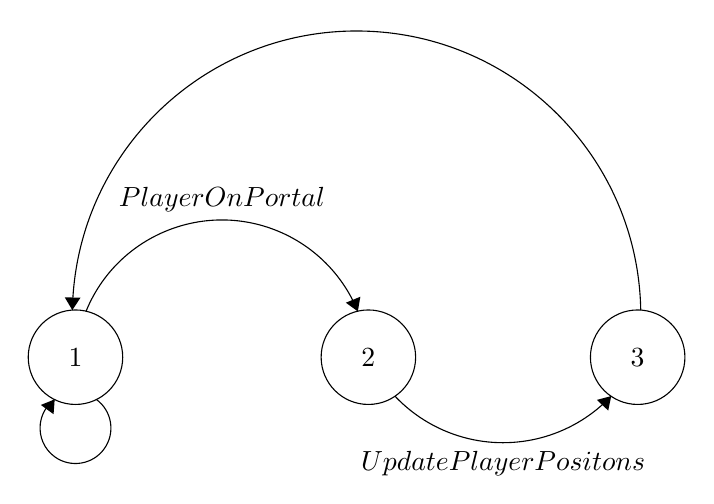
\begin{tikzpicture}[scale=0.2]
		\tikzstyle{every node}+=[inner sep=0pt]
		\draw [black] (11.7,-26.6) circle (3);
		\draw (11.7,-26.6) node {$1$};
		\draw [black] (30.3,-26.6) circle (3);
		\draw (30.3,-26.6) node {$2$};
		\draw [black] (47.4,-26.6) circle (3);
		\draw (47.4,-26.6) node {$3$};
		\draw [black] (12.369,-23.689) arc (157.83031:22.16969:9.32);
		\fill [black] (29.63,-23.69) -- (29.79,-22.76) -- (28.87,-23.14);
		\draw (21,-17.39) node [above] {$PlayerOnPortal$};
		\draw [black] (13.023,-29.28) arc (54:-234:2.25);
		\fill [black] (10.38,-29.28) -- (9.5,-29.63) -- (10.31,-30.22);
		\draw [black] (45.718,-29.069) arc (-43.35936:-136.64064:9.446);
		\fill [black] (45.72,-29.07) -- (44.81,-29.31) -- (45.53,-29.99);
		\draw (38.85,-32.53) node [below] {$UpdatePlayerPositons$};
		\draw [black] (11.505,-23.61) arc (-181.02525:-358.97475:18.048);
		\fill [black] (11.5,-23.61) -- (12.02,-22.82) -- (11.02,-22.8);
		\end{tikzpicture}
	\end{center}
	\medskip
	\textbf{Projectile updating after being fired:}
	\medskip
	\begin{center}
		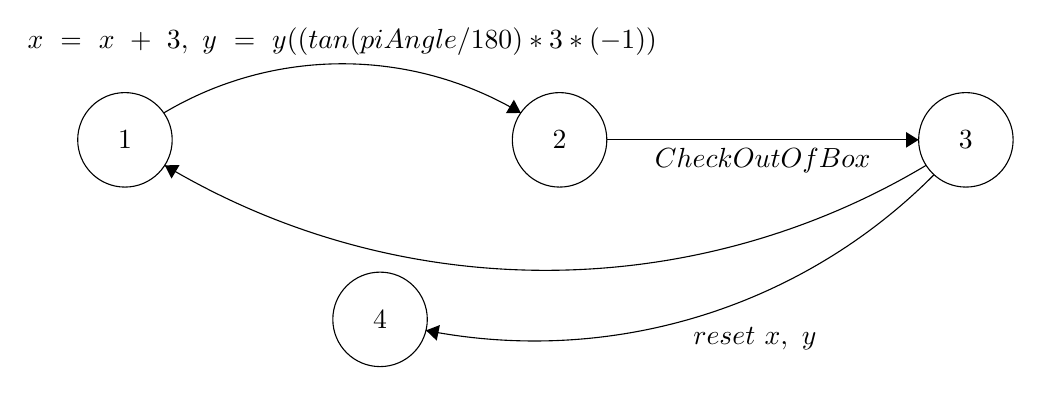
\begin{tikzpicture}[scale=0.2]
		\tikzstyle{every node}+=[inner sep=0pt]
		\draw [black] (9.2,-25.2) circle (3);
		\draw (9.2,-25.2) node {$1$};
		\draw [black] (36.8,-25.2) circle (3);
		\draw (36.8,-25.2) node {$2$};
		\draw [black] (62.6,-25.2) circle (3);
		\draw (62.6,-25.2) node {$3$};
		\draw [black] (25.4,-36.6) circle (3);
		\draw (25.4,-36.6) node {$4$};
		\draw [black] (11.665,-23.493) arc (120.816:59.184:22.127);
		\fill [black] (34.34,-23.49) -- (33.9,-22.65) -- (33.39,-23.51);
		\draw (23,-19.87) node [above] {$x\mbox{ }=\mbox{ }x\mbox{ }+\mbox{ }3,\mbox{ }y\mbox{ }=\mbox{ }y((tan(piAngle/180)*3*(-1))$};
		\draw [black] (39.8,-25.2) -- (59.6,-25.2);
		\fill [black] (59.6,-25.2) -- (58.8,-24.7) -- (58.8,-25.7);
		\draw (49.7,-25.7) node [below] {$CheckOutOfBox$};
		\draw [black] (60.578,-27.415) arc (-44.80789:-101.11658:35.756);
		\fill [black] (28.32,-37.3) -- (29,-37.95) -- (29.2,-36.96);
		\draw (49.2,-37.1) node [below] {$reset\mbox{ }x,\mbox{ }y$};
		\draw [black] (60.075,-26.819) arc (-59.15691:-120.84309:47.153);
		\fill [black] (11.73,-26.82) -- (12.16,-27.66) -- (12.67,-26.8);
		\end{tikzpicture}
	\end{center}
	\newpage
	\subsection{EFSM's}
	\textbf{Life reduction EFSM with movement and projectile movement:}
	\begin{center}
		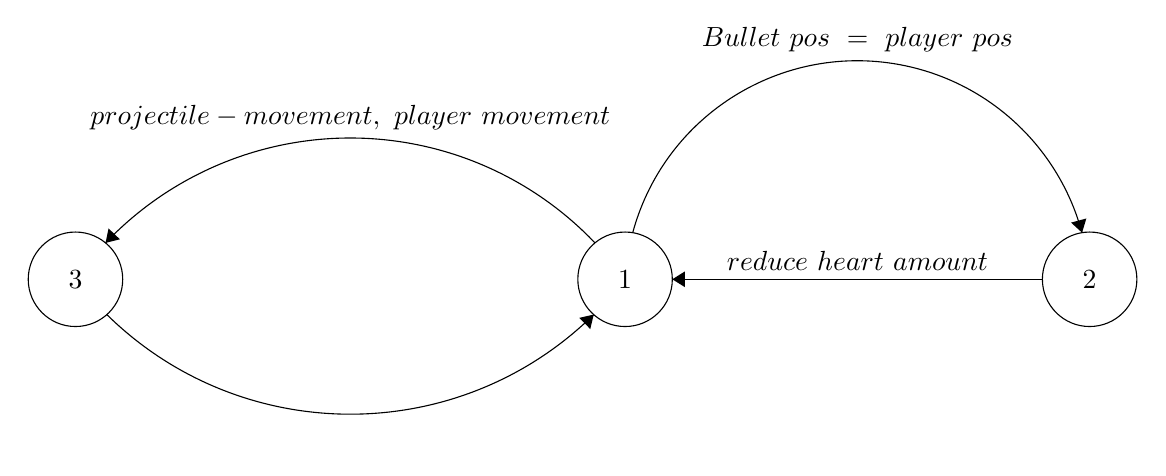
\begin{tikzpicture}[scale=0.2]
		\tikzstyle{every node}+=[inner sep=0pt]
		\draw [black] (42.2,-27.4) circle (3);
		\draw (42.2,-27.4) node {$1$};
		\draw [black] (71.7,-27.4) circle (3);
		\draw (71.7,-27.4) node {$2$};
		\draw [black] (7.3,-27.4) circle (3);
		\draw (7.3,-27.4) node {$3$};
		\draw [black] (42.685,-24.445) arc (164.86988:15.13012:14.778);
		\fill [black] (71.22,-24.44) -- (71.49,-23.54) -- (70.52,-23.8);
		\draw (56.95,-13.02) node [above] {$Bullet\mbox{ }pos\mbox{ }=\mbox{ }player\mbox{ }pos$};
		\draw [black] (9.21,-25.09) arc (136.40934:43.59066:21.456);
		\fill [black] (9.21,-25.09) -- (10.12,-24.86) -- (9.4,-24.17);
		\draw (24.75,-17.93) node [above] {$projectile-movement,\mbox{ }player\mbox{ }movement$};
		\draw [black] (40.21,-29.642) arc (-45.49754:-134.50246:22.056);
		\fill [black] (40.21,-29.64) -- (39.29,-29.85) -- (39.99,-30.56);
		\draw [black] (68.7,-27.4) -- (45.2,-27.4);
		\fill [black] (45.2,-27.4) -- (46,-27.9) -- (46,-26.9);
		\draw (56.95,-26.9) node [above] {$reduce\mbox{ }heart\mbox{ }amount$};
		\end{tikzpicture}
	\end{center}
	\subsection{Human Interface}
	The color background that we have decided to use makes it very easy to distinguish between the walls and the background. The bullet color and the enemy color was chosen to be red as it is the most commonly used color for dangerous objects, so that the player instinctively understands that they should avoid the bullets without being told to.
	\vspace{5mm}
	The star in the interface is also a universal symbol for an object that should be collected. Otherwise player may not know whether or not to move towards it. \\
	The hearts are placed at the top of the screen to be easily visible by the player.
	\section{Implementation}
	\subsection{Pre-conditions and Post-conditions}
	Write your subsection text here.
	\subsection{Specification vs Implementation}
	Write your subsection text here.
	\subsection{Side Effects}
	The lifebarchange funcion not only changes the amount of hearts the player currently has, but also the bullet class field has-hit, this is an example of where side effects can be very useful, when trigger-checks are updated so that they cannot be triggered again.
	\medskip
	The change function alters almost all the classes in the program, as well as our hash-table that is used for the movement and portal gun rotation. \\
	There are problems that come along with the change function have multiple side effects, such as the difficulty in locating problems in the code and what classes the issue is being created in.
	
	
	\section{Testing and Maintaining}
	\subsection{Test Cases and Assertions}
	\begin{itemize}
		\item test cases for movement
		\item test cases for teleporting through portals
		\item test cases for 
	\end{itemize}
	\subsection{User Feedback}
	survey-link here
	\begin{center}
		\begin{tabular}{ |c|c|c| } 
			\hline
			Animations & Color Scheme and Design & Fun and Overall Playability \\ 
			cell4 & cell5 & cell6 \\ 
			cell7 & cell8 & cell9 \\ 
			\hline
		\end{tabular}
	\end{center}
	
	\subsection{Subsection Heading Here}
	Interface requirements from survey results + fix.
	
	\section{Conclusion}
	Write your conclusion here.
	
\end{document}